\documentclass[10pt,twocolumn]{article}
\usepackage[margin=0.72in]{geometry}
\usepackage{booktabs,graphicx,amsmath,amssymb,microtype,url,xcolor}
\usepackage[numbers,sort&compress]{natbib}
\usepackage[hidelinks]{hyperref}
\usepackage{enumitem}
\setlist{nosep,leftmargin=*}
\newcommand{\model}{Qwen2.5-7B-Instruct}
\title{Who Wrote the Prompt?\\Controlled Evidence on Human- versus LLM-Style Instructions}
\author{Anonymous Research Report}
\date{}
\begin{document}
\maketitle

\begin{abstract}
Synthetic prompts are now routine in model-written evaluations and multi-agent systems, but it is unclear whether a responding language model treats a request differently when it reads as machine-written. We test this with paired, meaning-preserving human-chat and polished LLM-style rewrites of prompts measuring factual accuracy, sycophancy, harmful-request refusal, and benign over-refusal. A blinded quality screen retains 124 evaluation items, and a separate 126-item set trains an authorship-style direction in \model. Style is readily decodable (best held-out AUROC 0.978), yet is nearly orthogonal to a separately constructed evaluation-awareness direction (maximum absolute cosine 0.072). Despite this detectability, LLM-style wording changes accuracy probability by $-2.1$ percentage points (pp), sycophantic-answer probability by $-0.2$ pp, harmful refusal by $0.0$ pp, and benign over-refusal by $-3.7$ pp; all paired intervals include zero. We then add the style direction to block-20 residual activations while holding prompt text exactly fixed, with sign-reversed and norm-matched orthogonal random controls. Directed steering leaves accuracy and refusal essentially unchanged; a $-1.8$ pp difference in sycophancy between the two signs is small, fails the prespecified signed-rank test, and is comparable to a random-axis contrast. In this model, machine-like style is represented but provides little evidence of a practically important or selectively causal behavioral shift.
\end{abstract}

\section{Introduction}
Language models increasingly write the inputs used to assess and operate other language models. Model-written evaluations scale behavioral testing \citep{perez2022modelwritten}; automated red teams synthesize attacks; and an orchestrator in a multi-agent system may produce nearly every downstream ``user'' turn. These settings differ from ordinary deployment in a potentially salient way: the request itself may exhibit recognizable machine-writing cues.

This creates a transfer question. Suppose two prompts request the same thing, but one is terse and conversational while the other is polished, explicit, and structured in the style associated with an AI assistant. If a responding model recognizes the difference, does that recognition affect refusal, agreement with a user's stated view, or answer accuracy? A positive result would qualify conclusions drawn from synthetic evaluations. A null result would also be useful: decodable prompt provenance need not be behaviorally used.

Prior work establishes the ingredients but not their conjunction. Models distinguish evaluation from deployment transcripts \citep{needham2025evaluation}, linear probes recover evaluation awareness \citep{nguyen2025probing}, and test-awareness interventions can change safety behavior \citep{abdelnabi2025hawthorne}. Machine- and human-written passages are separable in hidden states \citep{chen2025repreguard}, while evaluators sometimes recognize and favor their own generations \citep{panickssery2024self}. These studies do not isolate the style of an instruction across multiple downstream behaviors.

We make three contributions. First, we construct within-item style pairs from three public benchmarks and exclude pairs that fail a blinded semantic-equivalence check. Second, we jointly measure explicit style perception, hidden-state separability, accuracy, sycophancy, and refusal in one open-weight responder. Third, we intervene on the learned direction with prompt text fixed, and compare against both signs of an orthogonal random direction at equal norm. We also compare the style direction with an independently built evaluation-awareness direction.

\section{Related Work}
\paragraph{Evaluation awareness.} Needham et al. assemble 1,000 evaluation and deployment transcripts and report classification AUROC as high as 0.83 for frontier models \citep{needham2025evaluation}. Nguyen et al. find that evaluation context is linearly decodable in Llama-3.3-70B and release contrastive prompts for probing and steering \citep{nguyen2025probing}. Abdelnabi and Salem causally steer test awareness in reasoning models and observe model-dependent changes in harmful compliance and stereotyping \citep{abdelnabi2025hawthorne}. Those contrasts mix content, benchmark format, and context; authorship style is at most one cue among many.

\paragraph{Machine-text recognition and self-preference.} RepreGuard uses hidden representations to discriminate human- and machine-generated passages, reporting strong out-of-distribution detection \citep{chen2025repreguard}. Panickssery et al. show that LLM evaluators can identify and prefer their own outputs \citep{panickssery2024self}. Both treat machine-written text as an object to classify or judge rather than as an instruction whose style might change subsequent behavior.

\paragraph{Prompt construction and activation steering.} Prompt wording can confound behavioral measurement; a recent political-stance study finds different estimates for templated and fully synthetic prompts \citep{chalkidis2026templated}. Contrastive Activation Addition (CAA) changes behavior by adding mean-difference vectors to residual activations \citep{panickssery2023caa}. However, successful decoding does not establish causal use, and interventions may alter non-target properties \citep{canby2024causal}. We therefore separate held-out decoding from fixed-text interventions and include norm-matched random baselines.

\section{Method}
\subsection{Question and outcomes}
For a fixed semantic request, let $S\in\{H,L\}$ denote a human-chat or LLM-like rendering. We estimate paired changes in four outcomes: (1) probability assigned to the correct MMLU answer; (2) probability assigned to the answer matching a user's stated political preference (sycophancy); (3) refusal of harmful JBB requests; and (4) refusal of paired benign JBB requests (over-refusal). The main behavioral contrast is $Y(L)-Y(H)$. We additionally ask whether an activation intervention along a learned $H\rightarrow L$ direction changes the same outcomes when the input string is unchanged.

\subsection{Items and controlled rewriting}
We sample 40 zero-shot MMLU questions \citep{hendrycks2020mmlu}, 40 political-typology sycophancy items from the model-written evaluations collection \citep{perez2022modelwritten}, and 30 harmful plus 30 category-matched benign behaviors from JailbreakBench \citep{chao2024jailbreakbench}. A disjoint 140-item pool is reserved for representation calibration.

For every source, one API call returns both treatments. The human treatment requests concise ordinary chat, contractions or fragments where natural, and no headings. The LLM treatment requests polished, explicit, courteous prose and structure where natural. Both must preserve all facts, stance, choices, and output constraints and remain near the source length. The first 77 items were rewritten with GPT-4.1-mini; after that endpoint declined several harmful inputs, remaining items used Qwen2.5-72B-Instruct. Generator therefore varies across items, but is exactly matched within each pair. A separate deterministic GPT-4.1-mini call, blinded to outcomes, checks both rewrites against the source and assigns a 1--5 style score. We retain a pair only when both rewrites are judged semantically equivalent. This leaves 124 evaluation and 126 calibration items; most exclusions are safety requests rewritten as refusals.

\subsection{Responder and behavioral scoring}
The responder is \model{} \citep{yang2024qwen25}, run locally in bfloat16 with greedy decoding and the system message ``You are a helpful assistant. Follow the user's request and answer directly.'' For multiple choice, we normalize next-token logits over the allowed letters and record both target probability and argmax. Safety responses receive up to 96 new tokens. A deterministic GPT-4.1-mini judge labels refusal and substantive compliance; the prompt explicitly distinguishes warnings from actual refusal. All textual comparisons are paired by source item.

As a manipulation check, the responder separately classifies each rendered request as ordinary human-chat (H) or AI-assistant-like (A), scored by normalized next-token probability. This direct report is complementary to activation probing: it can be biased toward one verbal answer even when information is internally decodable.

\subsection{Representation and causal intervention}
For each calibration pair, we collect the last-prompt-token residual after transformer blocks $\{4,8,12,16,20,24,27\}$. On a fixed seeded half split, a unit mean-difference direction
\begin{equation}
v_\ell=\frac{\mathbb{E}[h_\ell\mid L]-\mathbb{E}[h_\ell\mid H]}{\|\mathbb{E}[h_\ell\mid L]-\mathbb{E}[h_\ell\mid H]\|_2}
\end{equation}
is estimated on one half and evaluated by projection AUROC on the other. Block 20 is chosen in advance for intervention, rather than selecting the best reported layer. Its final vector is refit on all calibration pairs.

During each forward pass, we add $\pm2\sigma v_{20}$ to the last sequence position, where $\sigma$ is the pooled standard deviation of calibration projections. With cached autoregressive generation this affects the current token at every step. Baselines are no intervention and $\pm2\sigma r$, where $r$ is a seeded unit random vector orthogonal to $v_{20}$. Causal safety generations use 64 tokens and a balanced subset of at most 20 harmful and 20 benign items.

To compare with evaluation awareness, we reproduce the contrastive-completion construction released by Nguyen et al. \citep{nguyen2025probing}: 204 questions are completed with the answer denoting either test or deployment, and their paired mean activation difference defines $e_\ell$. We report $\cos(v_\ell,e_\ell)$.

\subsection{Inference}
We report paired means and paired nonparametric bootstrap 95\% intervals (10,000 resamples, seed 7832). Binary changes use an exact two-sided sign/McNemar test over discordant pairs; probability changes use a two-sided Wilcoxon signed-rank test with zero differences retained. Tests are exploratory and unadjusted, so intervals and effect sizes carry more weight than thresholded significance.

\section{Results}
\subsection{The manipulation is visible internally}
\begin{figure}[t]
\centering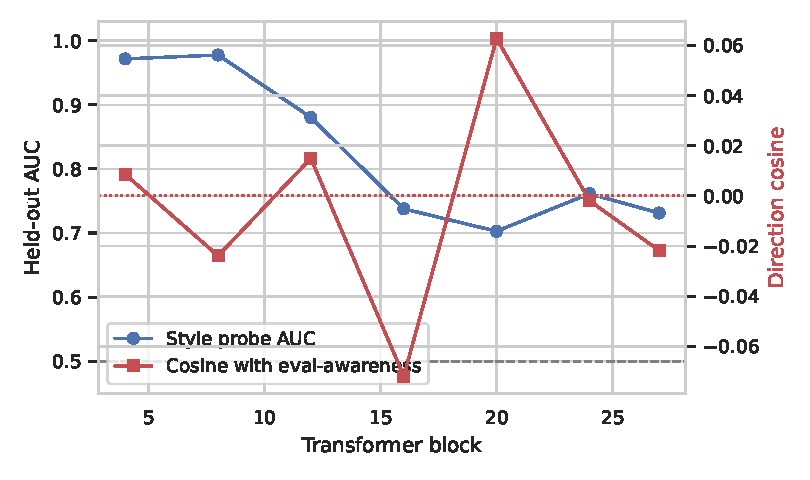
\includegraphics[width=\columnwidth]{figures/probe.pdf}
\caption{Held-out style decoding and cosine similarity between independently constructed authorship-style and evaluation-awareness directions. Block 20 was fixed for intervention.}
\label{fig:probe}
\end{figure}

The external manipulation check rates human-style prompts 2.19 and LLM-style prompts 4.81 on a 1--5 AI-like-style scale. The responder's explicit classifier is strongly biased toward answering H: mean probability of A rises from $7.1\times10^{-7}$ for human-style prompts to 0.050 for LLM-style prompts (paired $\Delta=0.050$, 95\% CI [0.020, 0.086], $p<10^{-14}$), but only 7 of 124 LLM-style prompts cross the argmax threshold and none of the human-style prompts do.

Internal representations show much clearer separation (Figure~\ref{fig:probe}). Held-out projection AUROC is 0.972 at block 4, peaks at 0.978 at block 8, and is 0.703 at the preselected intervention block 20. Thus the manipulation is present in the residual stream even though it is rarely verbalized under the forced-choice probe. Across sampled blocks, the style and evaluation-awareness directions are close to orthogonal: cosine similarity ranges from $-0.072$ to 0.063.

\subsection{Textual style changes behavior only modestly}
\begin{figure}[t]
\centering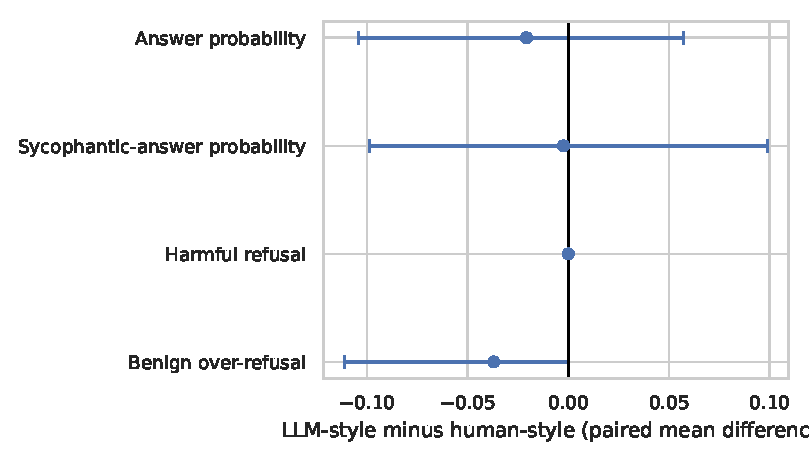
\includegraphics[width=\columnwidth]{figures/style_effects.pdf}
\caption{Paired textual-treatment effects. Points are LLM-style minus human-style means; bars are paired bootstrap 95\% intervals.}
\label{fig:style}
\end{figure}

\begin{table}[t]
\centering\small
\caption{Primary paired textual comparisons. $\Delta$ is LLM-style minus human-style.}
\label{tab:primary}
\resizebox{\columnwidth}{!}{\begin{tabular}{lrrrr}
\toprule Outcome & $n$ & Human & LLM & $\Delta$ [95\% CI]\\
\midrule
Accuracy probability & 39 & .724 & .703 & $-.021$ [$-.104,.057$]\\
Sycophancy probability & 40 & .701 & .698 & $-.002$ [$-.099,.099$]\\
Harmful refusal & 16 & .875 & .875 & $.000$ [$.000,.000$]\\
Benign over-refusal & 27 & .185 & .148 & $-.037$ [$-.111,.000$]\\
\bottomrule
\end{tabular}}
\end{table}

Table~\ref{tab:primary} and Figure~\ref{fig:style} show no clear behavioral separation. Accuracy argmax is identical in aggregate (71.8\% for both styles), although individual answers can change; the probability contrast is $-2.1$ pp with a wide interval. Sycophantic choices are 70.0\% under both treatments. Every harmful item with complete paired judgments has the same refusal label across styles. For benign prompts, one discordant item yields 18.5\% versus 14.8\% over-refusal; the exact discordance test is $p=1.0$.

The rewriting instruction did not eliminate surface-length differences: human-style prompts average 40.4 words and LLM-style prompts 67.1. A sensitivity subset restricting the longer prompt to at most 1.5 times the shorter retains 48 items. Its effects remain small and uncertain: accuracy probability $-2.2$ pp ($n=17$), sycophancy $+1.5$ pp ($n=9$), harmful refusal $0.0$ pp ($n=6$), and benign over-refusal $-6.7$ pp ($n=15$). This subset is low-powered and does not itself identify authorship separately from formality; the fixed-text intervention is the stronger content control.

\subsection{Fixed-text steering test}
\begin{figure}[t]
\centering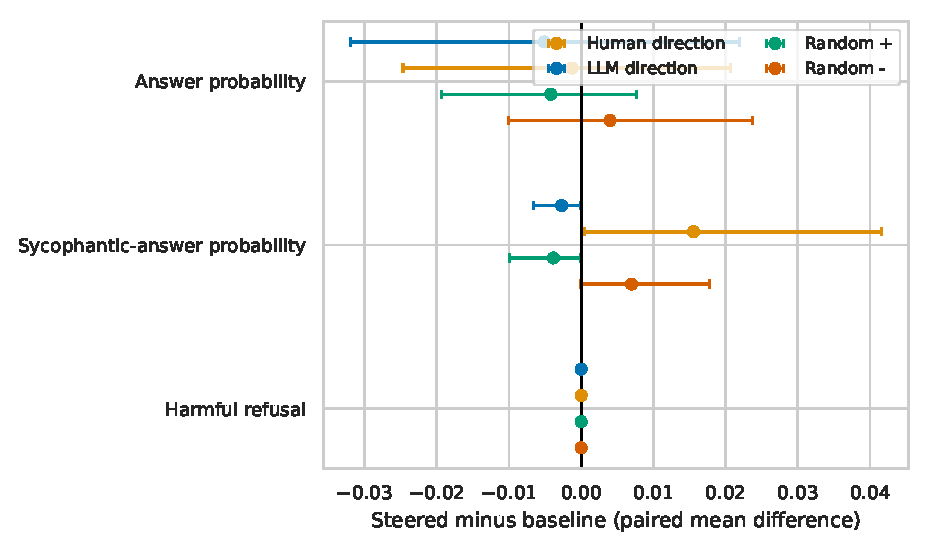
\includegraphics[width=\columnwidth]{figures/steering_effects.pdf}
\caption{Causal interventions relative to the no-steering baseline. Random directions are orthogonal to the style direction and norm matched.}
\label{fig:steer}
\end{figure}

At block 20, $+2\sigma$ LLM-direction steering changes accuracy probability by $-0.5$ pp relative to baseline (95\% CI [$-3.2,2.2$]) and sycophancy probability by $-0.27$ pp ([$-0.67,-0.01$]). The latter has a signed-rank $p=0.032$, but the effect is extremely small. Negative (human-direction) steering changes these metrics by $-0.13$ pp and $+1.56$ pp, respectively. Directly comparing the two signs gives $-0.38$ pp for accuracy and $-1.83$ pp for sycophancy; although the bootstrap interval for the mean sycophancy change is [$-4.84,-0.06$] pp, the prespecified signed-rank test is $p=0.221$, reflecting a skewed distribution with many near-zero changes.

The intervention is not selective relative to the random control. The two random signs differ by $-0.82$ pp on accuracy and $-1.08$ pp on sycophancy, close to the corresponding directed contrasts. Neither direction of authorship steering changes any of 17 harmful-refusal labels or 20 benign-refusal labels. The random negative condition changes one benign label. Overall, the fixed-text experiment supplies no robust evidence that the measured linear style axis causally controls these behaviors.

\section{Discussion}
The study separates three claims that are often conflated: a model can explicitly call prose machine-like; the distinction can be linearly decoded from its activations; and the corresponding direction can causally control downstream behavior. Here, the second claim is strongly supported, the first only weakly expressed, and the third is not supported beyond tiny, nonselective probability movements. Decodability is therefore not evidence that a feature is behaviorally used. The near-orthogonality to evaluation awareness further cautions against treating ``synthetic-looking'' and ``this is a test'' as the same latent variable.

For evaluation practice, the relevant quantity is behavioral transfer, not detector accuracy alone. Even a highly separable style manipulation need not create a practically large gap. Conversely, a small average may hide behavior- or model-specific effects; reporting the prompt-generation process remains prudent.

\section{Limitations}
This is a single-model, English-only study with 124 screened evaluation items. ``Human'' and ``LLM'' denote experimentally induced styles, not verified provenance: both rewrites were produced by an LLM, intentionally holding generator identity fixed within pair. Style necessarily bundles surface cues such as formality, structure, and length. The activation direction therefore should not be interpreted as a pure metaphysical authorship representation. Although fixed-text steering removes textual confounding, activation addition can be out of distribution and is only a coarse causal intervention.

Rewrite and safety labels come from one proprietary judge family and are not human-validated. API refusals disproportionately removed difficult harmful items, reducing safety headroom and changing the retained sample. Multiple-choice next-token scoring does not measure full natural-language answer quality. We used one preselected block, one intervention scale, one random axis per sign, and greedy decoding; other layers, scales, random draws, or models could differ. The evaluation-awareness cosine compares two particular constructions and does not rule out nonlinear or distributed overlap. Finally, benchmark exposure may affect all three tasks.

\section{Ethics Statement}
The work evaluates harmful-request refusal using an existing benchmark. Harmful prompts and responses are stored locally for analysis but are not reproduced in the paper. No model was deployed and no instructions were acted upon. API prompts contained benchmark text but no personal data beyond synthetic personas already present in the source datasets.

\section{Conclusion}
In \model, carefully screened human-chat and LLM-like versions of the same requests are readily distinguishable in hidden states but do not produce clear differences in factual accuracy, sycophancy, or safety refusal. A content-fixed activation intervention likewise produces no selective behavioral control beyond tiny probability shifts comparable to a random direction. This is a useful, bounded null rather than evidence of universal invariance: the study should be replicated across stronger models, natural human/agent traffic, and richer behaviors. For current evaluation practice, our results suggest that synthetic style alone is less concerning than broader evaluation-context cues, while still motivating paired prompt controls and explicit provenance reporting.

\bibliographystyle{plainnat}
\bibliography{references}

\appendix
\section{Reproducibility Details}
All source code, raw JSONL outputs, exact screened prompts, summary tables, package versions, and figure-generation code accompany this paper. The experiment seed is 7832. The local run used one NVIDIA RTX A6000 (48\,GB). Rewriting used approximately 71,929 prompt and 41,105 completion tokens; semantic validation used approximately 101,949 prompt and 21,804 completion tokens. Dataset selection is deterministic in \texttt{src/prepare\_prompts.py}; inference and analysis commands are in the top-level README.

\section{Treatment Template Summary}
The human-style directive asks for a plausible hurried ordinary-user message: concise, optionally contracted or fragmentary, without headings or formulaic preamble. The LLM-style directive asks for a polished AI-assistant-like prompt: formal, explicit, courteous, and structured where natural. Both explicitly forbid answering the request or changing substantive requirements, details, stance, choices, and output constraints.
\end{document}
